\chapter{Background}
\begin{quotation}
\noindent ``\emph{quote}''
\begin{flushright}\textbf{auteur, date}\end{flushright}
\end{quotation}

\vspace*{0.5cm}

\section{Machine Learning}
One could trace back the birth of the machine learning idea to Alan Turing's 
seminal paper, \textit{Computing Machinery and Intelligence} 
\cite{turing1950computing}. Although the computer science context around his
work was largely inexistent (at least compared to today), Turing already felt
the need to think of ways to transcend the fixed set of rules a computer had
to interpret and execute. As computer science grew, and as the field of
artificial intelligence went through its ebbs and flows throughout the years,
machine learning evolved from an idea to a prolific field of research, and
some of its topics saw massive application into real world domains.\\

The most popular and widely used machine learning algorithms and techniques
usually come from what we call supervised and unsupervised machine learning.
The broad goal of supervised machine learning is to find a function that maps
some input vector $x$ to some output vector $y$. One example of this would be
to try to categorise patients that either have or don't have some disease. 
The input vector $x$ could contain measurements such as blood pressure, the 
quantity of a given substance in the patient's blood, etc. The output vector
$y$ would be either $[0]$ if the patient is ill, and $[1]$ if the patient is
not.\\

If we could find a function mapping $x$ to $y$, we could predict to some
level of accuracy if a patient is ill or not by only knowing $x$. The general
algorithm for finding such a function is to define a model which has
\textit{learnable parameters}; that is values which impact the output of the
function, and to perform \textbf{training}. The process of training is to
sample one data point from a \textbf{training set}, containing pairs of input
vectors and output vectors. We then feed the input vector to our model, compare
the output that we get from the model with the output we are supposed to get,
and tune our learnable parameters so to minimise the error between the model
output and the correct output. We repeat this process, showing many samples
of the training set to our model until it reaches a good enough accuracy.

Unsupervised learning, although different from supervised learning as the
training sets usually do not have output vectors, is more about finding
structure in the dataset; but we can assume for the sake of this point that
the process is largely the same.\\

To the critical reader, unsupervised machine learning and supervised machine
learning might sound like fancy names for statistics; and one could argue that
they are indeed. Perhaps a slightly more interesting topic of machine learning
would be \textbf{reinforcement learning}. In this setting, we train an agent, 
which is situated in an environment, to perform actions that will maximise
a reward given by the environment.\\

This process works by letting the agent interact with the environment for many
sessions, until it figures out what actions, and what sequences of actions lead
to high rewards. This is the training process of a reinforcement learning agent.
One example of this is the CartPole problem \cite{barto-cartpole} where the
agent controls a cart on which a pole is balanced. The goal is to keep the
pole balanced for as long as possible by nudging the cart left or right. The
agent receives the position of the cart, the velocity of the cart, the pole
angle and the pole velocity at tip as a state observation from the environment,
and has to push the cart either left or right. The agent will first perform
randomly, but sooner or later, it will figure out how to balance the pole.\\

One common issue between all of the techniques described above is that once
training is over, the behaviour of the trained agent or model will not change
or adapt once the conditions, or some intrinsic parameters of the problem
change. If we present the CartPole agent with a pole that is twice as heavy,
or twice as long as the one it has been trained with, it will likely fail to 
balance the pole. We have taught an agent how to solve one task, but we have
not taught it to learn how to solve a task. The agent that has been trained is
not a learning agent. This thesis will explore ways to teach an agent to learn
to solve tasks.

\section{The reinforcement learning problem}
Reinforcement learning is a field of machine learning inspired by psychology.
It studies how an agent learns to maximize the cumulative reward it receives
from an environment in which it takes given actions.\\

\begin{figure}[]
	\centering
	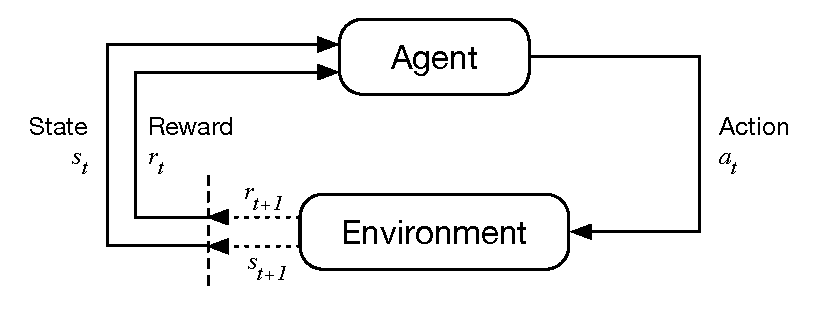
\includegraphics[width=0.65\linewidth]{fig/rl.eps}
	\caption{The setting of a reinforcement learning problem 
		\cite{suttonbarto}}
	\label{fig:rl}
\end{figure}

\subsection{Markov Decision Processes}
A reinforcement learning problem can be formally defined as a Markov 
Decision Process (MDP) \index{MDP} characterised by :
\begin{itemize}
	\item a set of states $\mathcal{S}$
	\item a set of actions $\mathcal{A}$
	\item a transition function 
		$T(s, a, s') = P(s_{t+1} = s' \mid s_t = s, a_t = a)$
	\item a reward function 
		$r(s, a, s') = \mathbb{E}
		 [r_{t+1} \mid s_t = s, a_t = a, s_{t+1} = s']$
\end{itemize}
For the rest of this paper, we will consider that the transition function is
deterministic.\\

The goal of reinforcement learning is for the agent to select, in any state it
can be in, the action that will lead it to the highest expected reward :

\begin{equation}
\mathbb{E}[r] = r_t + \gamma r_{t+1} + \gamma^2 r_{t+2}^2 + ... =
 \sum\limits_{i=0}^\infty \gamma^i r_{t+i}
\end{equation}

\noindent with the discount factor \index{discount factor} $\gamma \in [0, 1[$.
The discount factor allows one to tune the agent's behaviour on the
short-term/long-term spectrum. A discount factor $\gamma=0$ would mean that the
agent maximises its expected reward for the next transition only whereas a
discount factor close to one will favour behaviour that maximises long-term
reward, even if one action leads to a poor reward at first.\\

\subsection{Policy}
The agent uses a policy $\pi(a \mid s)$ which describes a probability
distribution over the action set $\mathcal{A}$, determining the probability of
selecting action $a_i$ from state $s_i$. This policy is 
\textbf{deterministic} if and only if :
\begin{equation}
\forall\, s \in \mathcal{S},\; \exists\, a \in \mathcal{A} : \pi(a \mid s) = 1
\end{equation}
\noindent Otherwise, the policy is \textbf{stochastic}.


\section{Neural networks as function approximators}
Neural networks have been very popular in the reinforcement learning community,
either to approximate a policy function or to approximate functions that
estimate the value of states and actions.\\

\subsection{Feedforward neural networks}
A neural network is a mathematical tool composed of three types of layers : 
the input layer, hidden layers and the output layer. Each layer is itself
composed of several "neurons".\\

In the simplest neural networks, such as the one presented in figure 
\ref{fig:neural_network}, each neuron in one layer is connected to all the
neurons of the previous layer. To obtain an output from a given input,
the information will be passed from layer to layer in the following way : 
each neuron calculates a weighted sum of the outputs of all neurons in the
previous layer then squashes this weighted sum in an activation function. 
Hence, the neuron $h_1$ in the network of figure \ref{fig:neural_network}
outputs:
$$ f(w_1i_1 + w_2i_2 + w_3i_3) $$
where $w_1, w_2, w_3$ are the weights corresponding to the connections between
$i_1, i_2, i_3$ and $h_1$. The activation function $f(\cdot)$ can be chosen 
arbitrarily but it is
the same for all the neurons in the same layer. The most popular options are
the sigmoid function, the hyperbolic tangent function and sometimes a linear
function.

A neural network is taught to approximate a function on a training
set of samples. Learning is performed by alternating feedforward passes and 
backpropagation, modifiying the weights of the connections between neurons until
the network reaches a satisfying accuracy.

\begin{enumerate}
	\item the feedforward pass computes the network output from the sample
		input data
	\item the network output is compared with the sample output and the
		error signal given by a loss function
		is backpropagated through the network, updating
		all the weights
\end{enumerate}

Backpropagation is a fundamental part of training a neural network but its
explanation is out of the scope of this work and we will assume that the
reader is at least somewhat familiar with it.

\begin{figure}[]
	\centering
	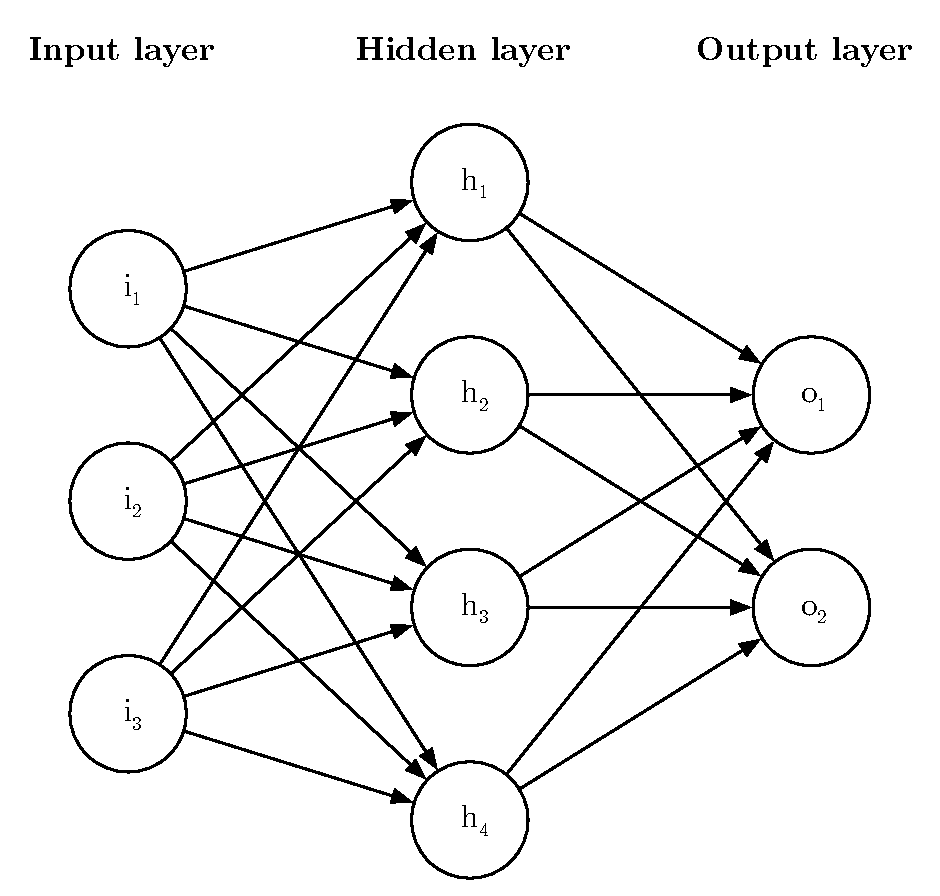
\includegraphics[width=0.6\linewidth]{fig/neural_network.eps}
	\caption{A neural network with one input layer composed of three neurons,
	one hidden layer of 4 neurons, and one output layer with 2 neurons.}
	\label{fig:neural_network}
\end{figure}


\subsection{Recurrent neural networks}
In some cases, it is a good idea to add a feedback loop to a neural network. 
A feedback loop such as the one shown in figure \ref{fig:rnn}, also called
a recurrent connection, poses evident issues for the backpropagation algorithm
since the depth of the neural network can become theoretically infinite.\\

A common way of training recurrent neural networks is to unroll them for a 
given, finite amount of time steps. The error signal can then be computed
for the output value at each time step, and backpropagated through all the
previous input values that affected its computing.\\

Recurrent neural networks are very useful in the context of reinforcement 
learning because they lay the ground for the memory aspect needed to solve
some tasks.

\begin{figure}[]
	\centering
	\subfloat[][A recurrent connection]{\qquad
		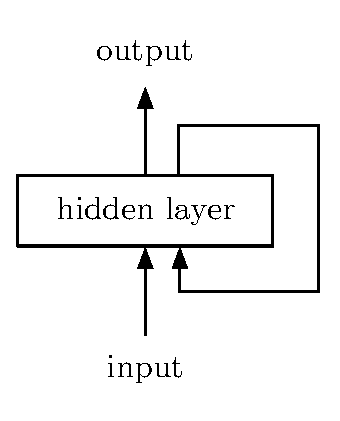
\includegraphics[width=0.1515\linewidth]{fig/recurrent_neural_network.eps}\qquad}
	\qquad
	\subfloat[][An unrolled recurrent neural network]{
		\includegraphics[width=0.6\linewidth]{fig/recurrent_neural_network_unrolled.eps}}
	\caption{Recurrent neural networks}
	\label{fig:rnn}
\end{figure}

\todo{universal function approximators}

\section{The A3C algorithm}
To understand A3C \cite{a3c}, which is one of the most popular reinforcement 
learning algorithms to date, one must first understand the two main groups of
reinforcement learning methods that sometimes intersect. The first is the 
group of policy gradient methods, and the second is the group of value 
methods.

\subsection{Policy gradient methods}
Policy gradient methods are rather straightforward ways of learning to solve a task.
Training starts with a randomly initialised policy. Let us assume that the
policy is defined by a neural network of which the input layer is set to 
receive an observation of the state of the environment. 
When the agent performs an action chosen with its policy, the environment will
update its state and the agent will receive an observation of this state as
well as a reward signal. We can use the reward signal to proportionately
encourage (if the reward is 
positive) or discourage (if the reward is negative) taking this action in 
this specific state. \\

Let $R_t$, the discounted future reward at time step $t$, be the metric
that we want to maximise. In a policy gradients method, we will update the
neural network policy directly with :
$$\alpha \nabla \pi(a \mid s) R_t$$
in which $\alpha$ is the learning rate.

\subsection{Value methods}
There is another category of methods which use an estimate of the value of
actions or states; in other words estimates of their discounted future reward
$R_t$.\\

The optimal state value function 
$$ V^*(s) = \mathbb{E}\left[ r_t + \gamma r_{t+1} + \gamma^2 r_{t+2}^2 + ...  \right]$$
can be estimated using the Bellman equation in the following way :
$$ V(s) = \mathbb{E}\left[ r_t + \gamma V(s')\right]$$
where $s'$ is the state reached after $s$.\\

Indeed, under the condition of optimality, the value of a state is the sum of
the discounted value of the unique optimal next state and the reward of the 
transition to that next state.\\

This can be used as an update rule for the $V$ network with a loss similar to :
$$ \left[V(s) -  \left(r_t + \gamma V(s') \right)\right]^2 $$

\paragraph{V, Q}

\subsection{Actor-Critic}



Advantage

